\chapter{Theoretical background}
In this section, I briefly introduce state-of-the-art methods and models used in experiment section. Many of the problems in NLP are tasks of mapping one sequence to another, therefore modern architectures were designed to tackle this very problem |\textbf{efficiently}.





\section{Text representation}
The NLP models operate on text on a \textbf{token} level. A token can be understood as the smallest unit of text and is a product of a process called \textbf{tokenization} (transforming text into set of tokens).

A common token unit is a word; however, tokens can be as small as a single byte. Currently, standard way of tokenization is using WordPiece tokens, which is a balance between word level and byte level tokenization.

After the tokenization, a numerical representation for the tokens has to be obtained. A naive way is to use mapping for every word to an index in predefined/obtained vocabulary. Such an approach suffers from the explicit ordering of the words, which may negatively influence the model. Another possible representation is the \textbf{one-hot-encoding} where each word is represented by a vector that has $1$ in a single row and zeros everywhere else. The size of such an encoding is proportional to the size of the vocabulary, making the feature space very sparse. 

The current standard representation of words are word \textbf{embeddings}. Embeddings are fixed-size feature vectors. The dimension of the embeddings is a hyperparameter, usually with the value between 100 and 1000. Embeddings are usually learned along the particular task, in an Embedding layer. But there are also precomputed representations available, such as word2vec, Glove or ELmo.
\newpage





\section{Neural Networks}
An \Gls{ann} is a model developed in the early 1940s. The smallest unit of a \Gls{nn} is a perceptron:
\begin{equation}
    f(x) = \phi(w^Tx + b)
\end{equation}
Where \textbf{weight} vector $w$ and \textbf{bias} term $b$ are learnable parameters, $x$ is an input feature vector and $\phi$ is an \textbf{activation function}. Activation functions are used for introducing non-linearities into the \Gls{nn}. In case of perceptron, it is a simple threshold function. Although the definition of \Gls{mlp} is loose, it can be understood as a simplest form of neural network with multiple connected perceptrons and a threshold activation function. In general, \Gls{nn}s usually use other activation functions such as sigmoid, ReLu, Tanh, LeakyReLu, etc.





\section{Encoder-Decoder}
Vanilla \Gls{nn} architecture operates on inputs of fixed length. For variable length (for example a sentence) input \Gls{rnn} is used. Let $x = (x_1,x_2,...,x_T)$ be the input sequence. \gls{rnn} works on $x$ sequentially, updating its \textbf{hidden state} vector $h$ with some non-linear function, such as sigmoid, at each discrete time step. The final hidden state, also called a \textbf{context vector} $c_T$, is preserved.
Therefore, \Gls{rnn} is able to map the input of arbitrary length $T$ to a fixed size vector $c_T$ that captures the information of the entire sequence.

Sequence-to-sequence \cite{sutskever2014sequence,cho2014learning} or \textbf{seq2seq} model aims to tackle the problem of mapping one sequence to another using two \Gls{rnn}s. The first \Gls{rnn} called \textbf{Encoder} is used to map the input sequence of arbitrary length to the fixed-size context vector. The context vector is then fed to a second \Gls{rnn} called \textbf{Decoder}. The decoder processes the context vector to a final sequence $y = (y_1,...,y_k)$, by updating its hidden state vectors while generating outputs $y_t$.

There are several problems with this architecture. Firstly, when a long sequence is processed, the information from earlier parts of sequence is "forgotten". Secondly, RNNs work in a sequential manner, hence there is no room for parallelism. A \textbf{Transformer} architecture aim to solve these problems.





\section{Transformers}\label{att_transformers}
Transformers is a family of deep neural architectures, that has revoulutionized an \gls{nlp} field. The \textbf{attention} mechanism is a core principle behind inside transformer architecture and solves some of the problems mentioned in previous section.

Current \gls{sota} language models, such as GPT-3, BERT, RoBERTa all use this architecture with different modifications (eg., BERT only uses the encoder side etc). For detection of media bias, I have eventually also narrowed the choice of models to transformers rather than other neural architectures.



\subsection{Attention}
Attention \cite{bahdanau2014neural,luongeffective} is essentially a mechanism that alows the unit (either it is on the decoder or the encoder side) to learn to focus on some segments of input sequence more than the others. This mechanism has been motivated by the problem of "forgetting" of information in a long sequences mentioned before. This way, parts of the sequences that potentially drives the decision are represented more in hidden states than other parts.

\begin{figure}
  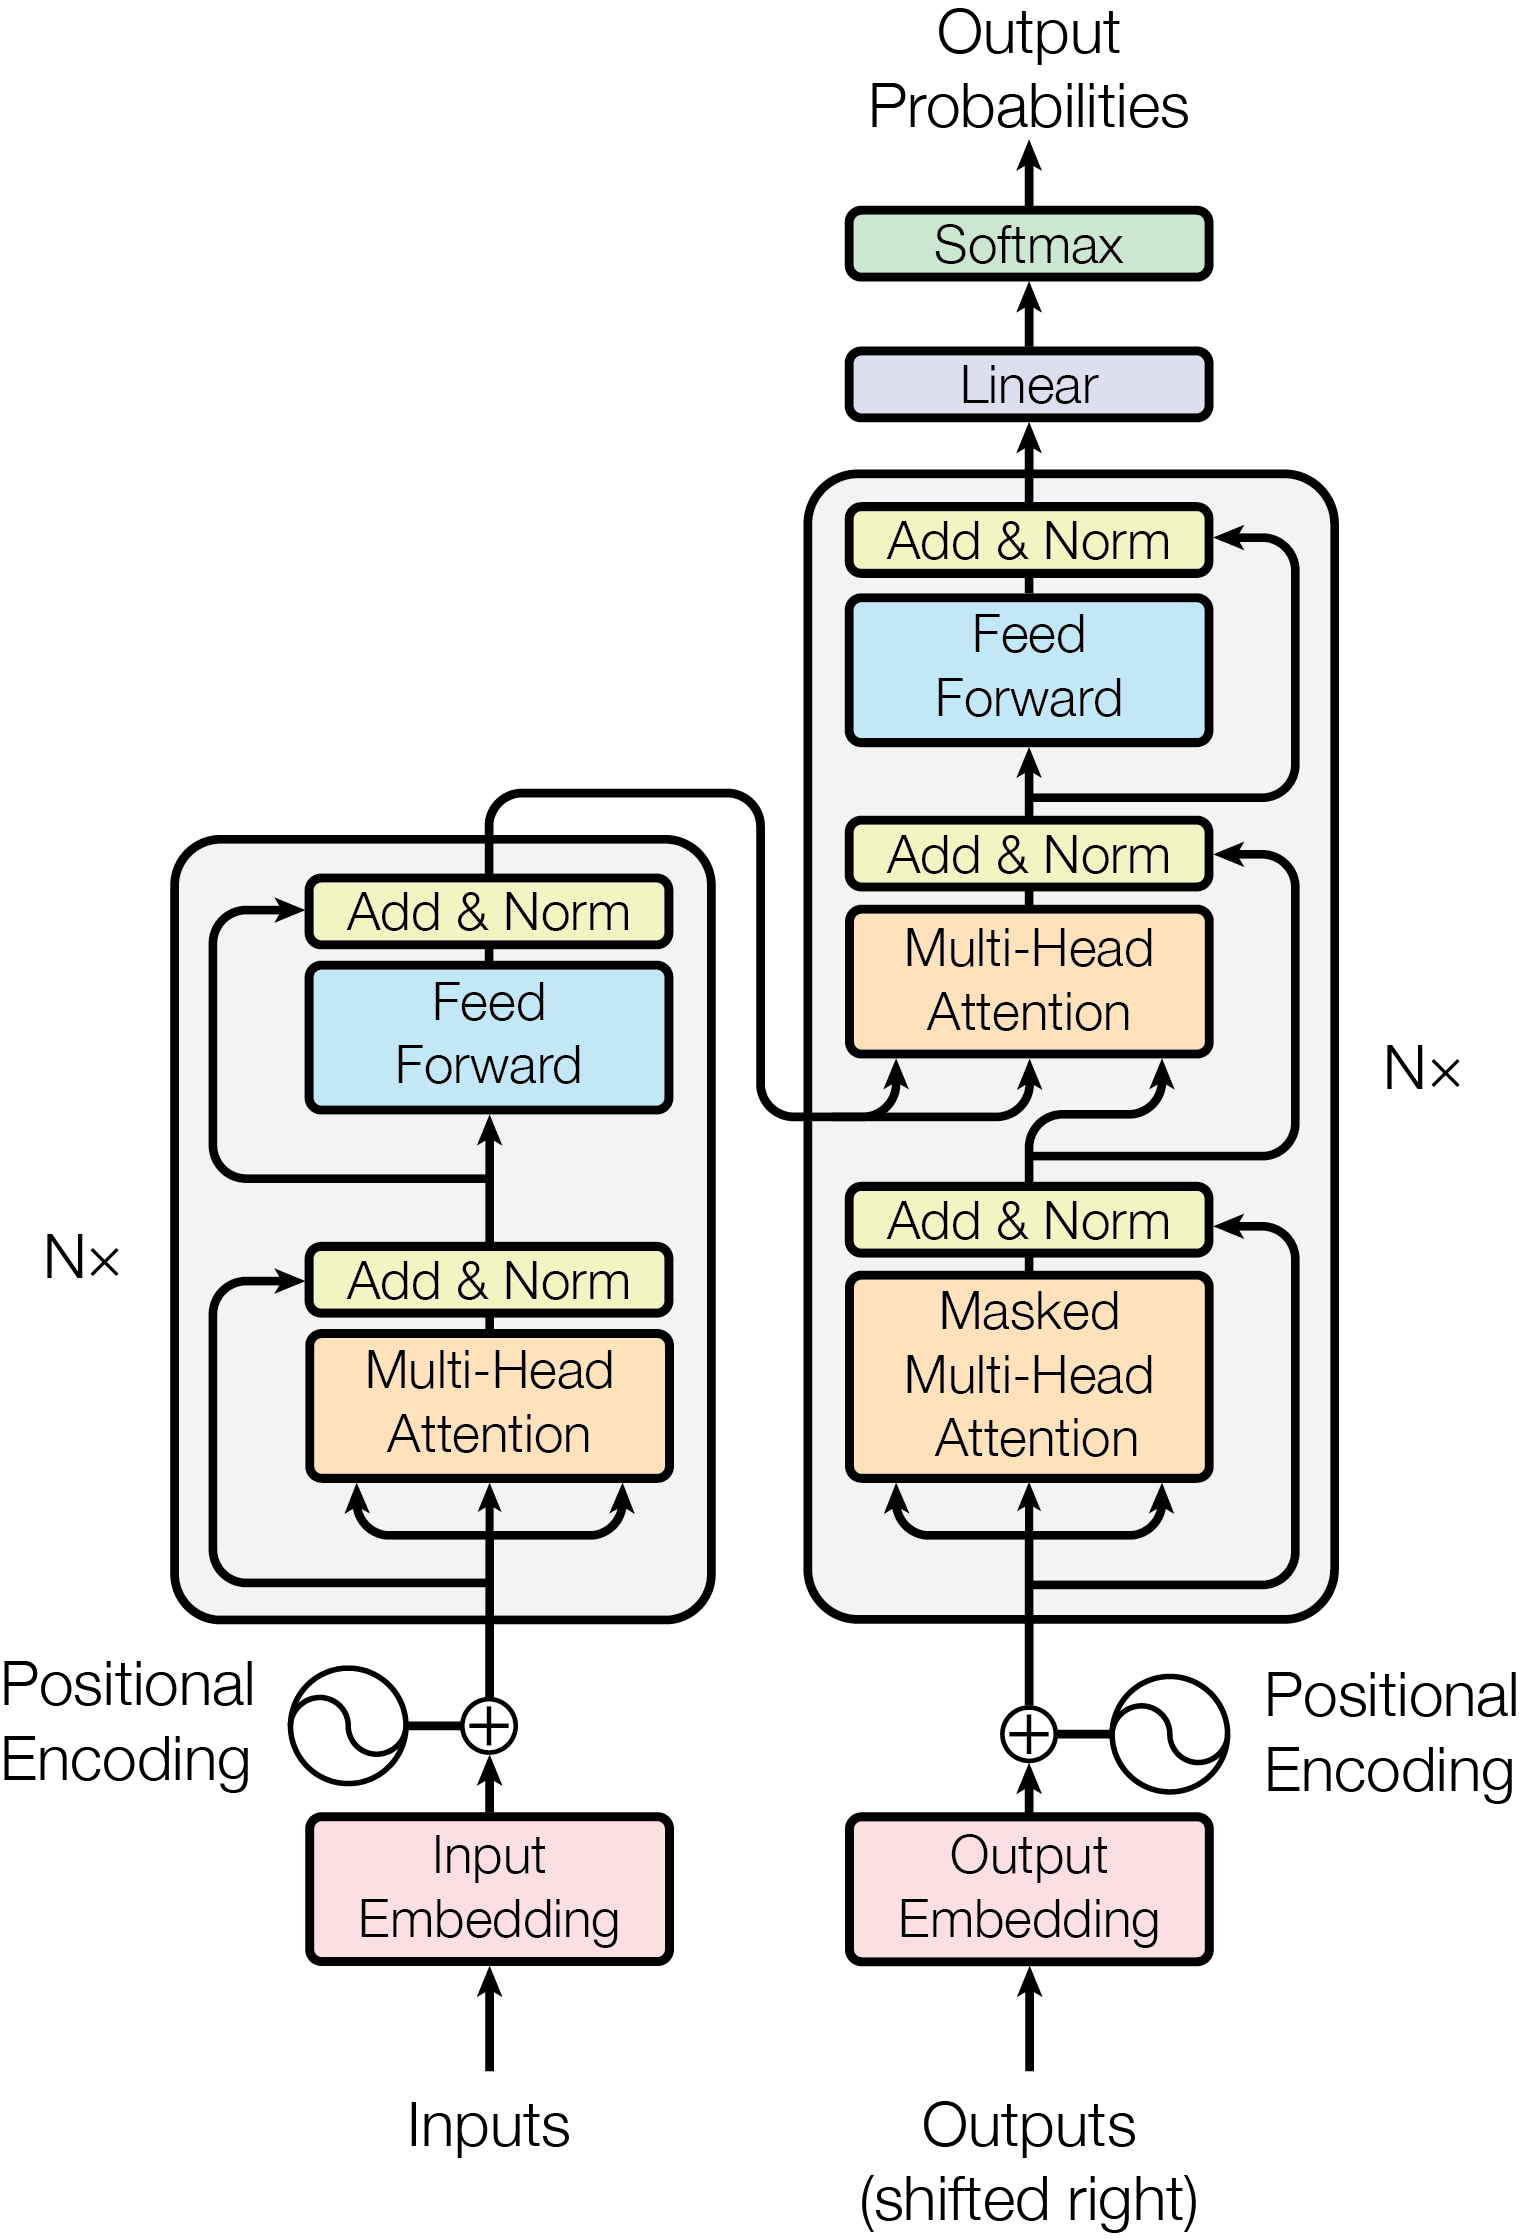
\includegraphics[scale=0.5]{my_modules/multimedia/atalyned.png}
  \caption{Transformer model architecture, preprinted reprinted from \cite{vaswani2017attention}}
  \label{fig:transformer}
\end{figure}

\subsection{Transformer architecture}
Scheme of the original architecture can be seen in \ref{fig:transformer}. Just as previous seq2seq models, transformer also consists of Encoder and Decoder modules. Precisely, each module is a stack of $n$ identical encoder or decoder layers.

Each encoder layer 

Instead of working on each token sequentially (as conventional Encoder-Decoder did), transformer builds hidden state representations for all tokens in sequence in \textbf{parallel}.




\section{Text classification}
Text classification is a supervised learning task of assigning a particular text (word, sentence, or document) a category to which it belongs to. A standard loss for classification is a Cross-Entropy loss. In case of binary classification:

\begin{equation}
    L_{BCE} = \frac{1}{n} \sum_{i=1}^n ( y_i \cdot \log\hat{y_i} + (1-y_i)\cdot(1-\hat{y_i}))
\end{equation}

where $y_i$ denotes the ground-truth label, $\hat{y_i}$ the probability predicted by the model, and $n$ is a number of samples.


    
\subsection{Metrics}
The most straight-forward way to evaluate the prediction ability of a classifier is to use \textbf{accuracy} metric, which means counting correctly classified  data. 
\begin{equation}
    accuracy = \frac{correct\ predictions}{total\ predictions}
\end{equation}
This metric is feasible if classes of the dataset are balanced. However, imagine a situation where 90\% of data belong to one class and only 10\% to another. Classifier, that always outputs the first class, achieves 90\% accuracy even though its prediction capability is trivial. For unbalanced data, it is convenient to use the \textbf{F1} metric. The F1 score is a harmonic mean of \textit{Precision} and \textit{Recall}.

\begin{equation}
    F1 = \frac{2*Precision*Recall}{Precision + Recall}
\end{equation}
where precision

\begin{equation}\footnote{TP,TN,FP,FN denotes to True positive, True Negative, Fasle Positive, False Negative respectively.}
    Precision = \frac{TP}{TP+FP}
\end{equation}
can be understood as "how precisely the model predicts a positive class", whereas recall
\begin{equation}
    Rrecall = \frac{TP}{TP+FN}
\end{equation}
can be understood as "how much of a positive class can model predict".
Scores for each class are then averaged to obtain the final score.




\subsection{Transformers for text classification}
Predictive power of transformers is behind every \gls{sota} result and text classification is no exception. For classification, usually only the Encoder part of a transformer is used, although some define the classification problem as a sequence-to-sequence and incorporate the decoder too \cite{raffel2019exploring}.

During tokenization, special [CLS] token is prepended to a sentence. The token has its own embedding and flows through the stack of encoders just as any other token, with the difference, that when the forward pass reaches the classification layer, only [CLS] token is passed as an input. [CLS] token can therefore be understood as sort of a sentence embedding.

Usually, one or two dense layers with activation function are sufficient as a classifier on top of encoder stack. However it is also possible to extract representations from any level of encoder stack and run arbitrary classification algorithm on top of it.




\section{Transfer learning}
Nowadays the true power of transformers lies in \textbf{transfer learning}. Transfer is a process when some knowledge is not learned from scratch but transfered from previously trained model. Since large language models such as BERT or RoBERTa has millions of parameters, it would be extremely costly to train them from scratch. 

Such large models are usually pretrained on a very large corpus of data. There are several common \textbf{unsupervised} pre-training tasks, that allow these models to learn contextual representations of words without supervision. For instance \gls{mlm} is a task, where random sample of tokens in input sequence is replaced with [MASK] token and model learns to predict the original token. Or \gls{nsp} which is self-explanatory.

Having such pre-trained model, one can then easily train a task specific head on top of pre-trained representations. Although process of \textbf{fine-tuning} where all parameter of model are tuned, is more often adopted.
